%\documentclass[landscape,a0b,final,a4resizeable]{a0poster}
\documentclass[portrait,a0b,final]{a0poster}
%\documentclass[portrait,a0b,final,a4resizeable]{a0poster}
%\documentclass[portrait,a0b,final]{a0poster}
%%% Option "a4resizeable" makes it possible ot resize the
%   poster by the command: psresize -pa4 poster.ps poster-a4.ps
%   For final printing, please remove option "a4resizeable" !!

\usepackage{epsfig}
\usepackage{multicol}
\usepackage{pstricks,pst-grad}
\usepackage{amsmath}

%\usepackage{algorithm}
%\usepackage{algorithmic}



%%%%%%%%%%%%%%%%%%%%%%%%%%%%%%%%%%%%%%%%%%%
% Definition of some variables and colors
%\renewcommand{\rho}{\varrho}
%\renewcommand{\phi}{\varphi}
\setlength{\columnsep}{3cm}
\setlength{\columnseprule}{2mm}
\setlength{\parindent}{0.0cm}



%%%%%%%%%%%%%%%%%%%%%%%%%%%%%%%%%%%%%%%%%%%%%%%%%%%%
%%%               Background                     %%%
%%%%%%%%%%%%%%%%%%%%%%%%%%%%%%%%%%%%%%%%%%%%%%%%%%%%

\newcommand{\background}[3]{
  \newrgbcolor{cgradbegin}{#1}
  \newrgbcolor{cgradend}{#2}
  \psframe[fillstyle=gradient,gradend=cgradend,
  gradbegin=cgradbegin,gradmidpoint=#3](0.,0.)(1.\textwidth,-1.\textheight)
}



%%%%%%%%%%%%%%%%%%%%%%%%%%%%%%%%%%%%%%%%%%%%%%%%%%%%
%%%                Poster                        %%%
%%%%%%%%%%%%%%%%%%%%%%%%%%%%%%%%%%%%%%%%%%%%%%%%%%%%

\newenvironment{poster}{
  \begin{center}
  \begin{minipage}[c]{0.98\textwidth}
}{
  \end{minipage} 
  \end{center}
}



%%%%%%%%%%%%%%%%%%%%%%%%%%%%%%%%%%%%%%%%%%%%%%%%%%%%
%%%                pcolumn                       %%%
%%%%%%%%%%%%%%%%%%%%%%%%%%%%%%%%%%%%%%%%%%%%%%%%%%%%

\newenvironment{pcolumn}[1]{
  \begin{minipage}{#1\textwidth}
  \begin{center}
}{
  \end{center}
  \end{minipage}
}



%%%%%%%%%%%%%%%%%%%%%%%%%%%%%%%%%%%%%%%%%%%%%%%%%%%%
%%%                pbox                          %%%
%%%%%%%%%%%%%%%%%%%%%%%%%%%%%%%%%%%%%%%%%%%%%%%%%%%%

\newrgbcolor{lcolor}{0. 0. 0.80}
\newrgbcolor{gcolor1}{1. 1. 1.}
\newrgbcolor{gcolor2}{.80 .80 1.}

\newcommand{\pbox}[4]{
\psshadowbox[#3]{
\begin{minipage}[t][#2][t]{#1}
#4
\end{minipage}
}}



%%%%%%%%%%%%%%%%%%%%%%%%%%%%%%%%%%%%%%%%%%%%%%%%%%%%
%%%                myfig                         %%%
%%%%%%%%%%%%%%%%%%%%%%%%%%%%%%%%%%%%%%%%%%%%%%%%%%%%
% \myfig - replacement for \figure
% necessary, since in multicol-environment 
% \figure won't work

\newcommand{\myfig}[3][0]{
\begin{center}
  \vspace{1.5cm}
  \includegraphics[width=#3\hsize,angle=#1]{#2}
  \nobreak\medskip
\end{center}}



%%%%%%%%%%%%%%%%%%%%%%%%%%%%%%%%%%%%%%%%%%%%%%%%%%%%
%%%                mycaption                     %%%
%%%%%%%%%%%%%%%%%%%%%%%%%%%%%%%%%%%%%%%%%%%%%%%%%%%%
% \mycaption - replacement for \caption
% necessary, since in multicol-environment \figure and
% therefore \caption won't work

%\newcounter{figure}
\setcounter{figure}{1}
\newcommand{\mycaption}[1]{
  \vspace{0.5cm}
  \begin{quote}
    {{\sc Figure} \arabic{figure}: #1}
  \end{quote}
  \vspace{1cm}
  \stepcounter{figure}
}



%%%%%%%%%%%%%%%%%%%%%%%%%%%%%%%%%%%%%%%%%%%%%%%%%%%%%%%%%%%%%%%%%%%%%%
%%% Begin of Document
%%%%%%%%%%%%%%%%%%%%%%%%%%%%%%%%%%%%%%%%%%%%%%%%%%%%%%%%%%%%%%%%%%%%%%

\begin{document}

\background{1. 1. 1.}{1. 1. 1.}{0.5}

\vspace*{2cm}


\newrgbcolor{lightblue}{0. 0. 0.80}
\newrgbcolor{white}{1. 1. 1.}
\newrgbcolor{whiteblue}{.80 .80 1.}


\begin{poster}

%%%%%%%%%%%%%%%%%%%%%
%%% Header
%%%%%%%%%%%%%%%%%%%%%
\begin{center}
\begin{pcolumn}{0.98}

\pbox{0.962\textwidth}{}{linewidth=2mm,framearc=0.3,linecolor=lightblue,fillstyle=gradient,gradangle=0,gradbegin=white,gradend=whiteblue,gradmidpoint=1.0,framesep=1em}{

%%% Unisiegel
\begin{minipage}[c][9cm][c]{0.1\textwidth}
  \begin{center}
    \includegraphics[angle=0,width=8cm]{images/hamilton-logo.epsi}
  \end{center}
\end{minipage}
%%% Titel
\begin{minipage}[c][9cm][c]{0.78\textwidth}
  \begin{center}
    {\sc \Huge Ambient Radiofrequency Power: the Impact of the Number of Devices in a Wi-Fi Network}\\[10mm]
    {\Large David Malone, Lesley A.~Malone\\[7.5mm]
    Hamilton Institute, National University of Ireland Maynooth. Clinical Medicine, Trinity College Dublin.}
  \end{center}
\end{minipage}
%%% GK-Logo
\begin{minipage}[c][9cm][c]{0.1\textwidth}
  \begin{center}
    
\includegraphics[width=7cm,angle=0]{images/NUIM_Logo.eps}
  \end{center}
\end{minipage}

}
\end{pcolumn}
\end{center}


\vspace*{2cm}



%%%%%%%%%%%%%%%%%%%%%
%%% Content
%%%%%%%%%%%%%%%%%%%%%
\begin{center}
\begin{pcolumn}{0.49}
\pbox{0.9\textwidth}{28cm}{linewidth=2mm,framearc=0.1,linecolor=lightblue,fillstyle=gradient,gradangle=0,gradbegin=white,gradend=white,gradmidpoint=1.0,framesep=1em}{
\medskip
%%% Abstract
\begin{center}\pbox{0.8\textwidth}{}{linewidth=2mm,framearc=0.1,linecolor=lightblue,fillstyle=gradient,gradangle=0,gradbegin=white,gradend=whiteblue,gradmidpoint=1.0,framesep=1em}{\begin{center}802.11 Networks\end{center}}\end{center}\vspace{1.25cm}


\begin{itemize}
\item Standard used for home/office wireless networks,
\item Branded as \emph{WiFi},
\item Uses ISM band at 2.4GHz (802.11b/g),
\item Or maybe at 5GHz (802.11a),
\item Transfers packets of data like Ethernet.
\item Carrier sense multiple access protocol.
\end{itemize}

\medskip

Aim: to calculate radiofrequency exposure bounds from large networks.

\medskip 

Complication: 802.11 MAC Layer, power is neither fixed nor simple scaling.

\begin{itemize}
\item After transmission choose rand(0,CW-1).
\item Wait until medium idle.
\item Count down in slots.
\item Transmit when get to 0 (if you have a packet).
\item If ACK then $CW \leftarrow CW_{min}$ else $CW \leftarrow 2CW$.
\end{itemize}


}
\end{pcolumn}
%%%%%%%%%%%%%%%%%%%%%%
%%%%%%%%%%%%%%%%%%%%%%
\begin{pcolumn}{0.49}
\pbox{0.9\textwidth}{28cm}{linewidth=2mm,framearc=0.1,linecolor=lightblue,fillstyle=gradient,gradangle=0,gradbegin=white,gradend=white,gradmidpoint=1.0,framesep=1em}{

\medskip
%%% Introduction
\begin{center}\pbox{0.8\textwidth}{}{linewidth=2mm,framearc=0.1,linecolor=lightblue,fillstyle=gradient,gradangle=0,gradbegin=white,gradend=whiteblue,gradmidpoint=1.0,framesep=1em}{\begin{center}802.11 MAC Layer\end{center}}\end{center}\vspace{1.25cm}

\smallskip

802.11 MAC is randomised: concurrent transmissions are possible.

\smallskip

\begin{center}
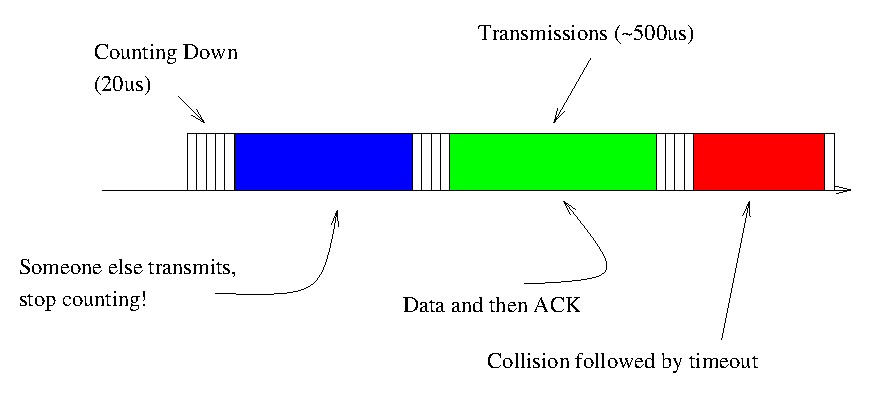
\includegraphics[width=37cm]{80211mac}
\end{center}

\smallskip


}
\end{pcolumn}
%%%%%%%%%%%%%%%%%%%%%%
\end{center}
%%%%%%%%%%%%%%%%%%%%%%

%%%%%%%%%%%%%%%%%%%%%%%%%%%%%%%%%%%%%%%%%%%%%%%%%%%%%%%%%%%%%%%%%%%%%%%%
% ROW 2                                                                %
%%%%%%%%%%%%%%%%%%%%%%%%%%%%%%%%%%%%%%%%%%%%%%%%%%%%%%%%%%%%%%%%%%%%%%%%
\vspace*{2cm}

%%%%%%%%%%%%%%%%%%%%%
%%% Content
%%%%%%%%%%%%%%%%%%%%%
\begin{center}
\begin{pcolumn}{0.49}
\pbox{0.9\textwidth}{28cm}{linewidth=2mm,framearc=0.1,linecolor=lightblue,fillstyle=gradient,gradangle=0,gradbegin=white,gradend=white,gradmidpoint=1.0,framesep=1em}{

\medskip
%%% Introduction
\begin{center}\pbox{0.8\textwidth}{}{linewidth=2mm,framearc=0.1,linecolor=lightblue,fillstyle=gradient,gradangle=0,gradbegin=white,gradend=whiteblue,gradmidpoint=1.0,framesep=1em}{\begin{center}Bianchi Models\end{center}}\end{center}\vspace{1.25cm}

\smallskip

Work by Bianchi in traffic engineering has allowed the probability:

\begin{itemize}
\item idle states,
\item successful transmissions,
\item collisions.
\end{itemize}

Data throughput then calculated as:

\begin{equation}
\frac{D_S n \tau ( 1 - \tau )^{n-1}}{T_I ( 1 - \tau )^n + T_S n \tau ( 1 - \tau )^{n-1} + T_C (1-( 1 - \tau )^n-n \tau ( 1 - \tau )^{n-1})}
\end{equation}

where $D_S$ is the amount of data in a successfully transmitted
packet and $T_I$, $T_S$ and $T_C$ are the times taken for an idle state,
a successful transmission and a collision respectively.

\medskip

We generalise to calculate probability of $r$ stations transmitting
at a time, and then calculate mean power as:
\begin{equation}
P = \frac{E}{T} = \frac{0 ( 1 - \tau )^n + E_S n \tau ( 1 - \tau )^{n-1} + E_C \sum_{r = 2}^{n} r \binom{n}{r} \tau^r (1-\tau)^{n-r}}{T_I ( 1 - \tau )^n + T_S n \tau ( 1 - \tau )^{n-1} + T_C (1-( 1 - \tau )^n-n \tau ( 1 - \tau )^{n-1}}.
\end{equation}
where $E_I$, $E_S$ and $E_C$ are the times taken for an idle state,
a successful transmission and a collision respectively.



}
\end{pcolumn}
%%%%%%%%%%%%%%%%%%%%%%
\begin{pcolumn}{0.49}
\pbox{0.9\textwidth}{28cm}{linewidth=2mm,framearc=0.1,linecolor=lightblue,fillstyle=gradient,gradangle=0,gradbegin=white,gradend=white,gradmidpoint=1.0,framesep=1em}{

\medskip
%%% Introduction
\begin{center}\pbox{0.8\textwidth}{}{linewidth=2mm,framearc=0.1,linecolor=lightblue,fillstyle=gradient,gradangle=0,gradbegin=white,gradend=whiteblue,gradmidpoint=1.0,framesep=1em}{\begin{center}Results: Saturated Unicast Traffic\end{center}}\end{center}\vspace{1.25cm}

\smallskip

\begin{center}
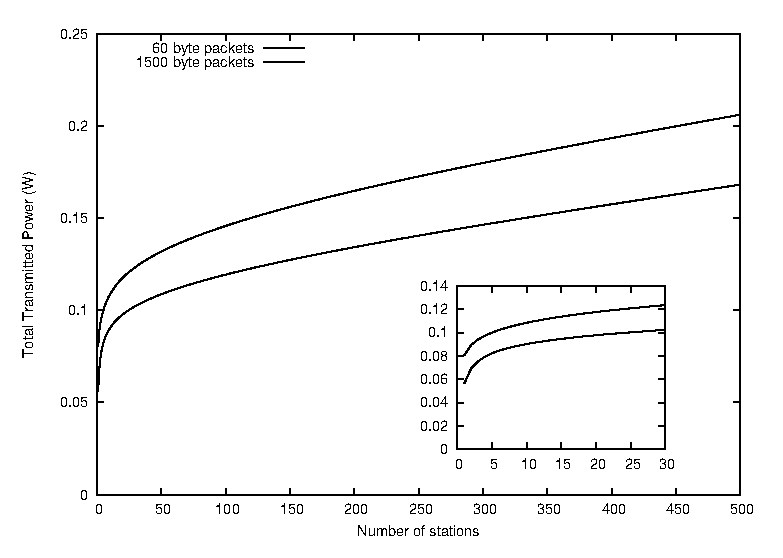
\includegraphics[width=30cm]{power1}
\end{center}


}
\end{pcolumn}
%%%%%%%%%%%%%%%%%%%%%%
\end{center}
%%%%%%%%%%%%%%%%%%%%%%%%%%%%%%%%%%%%%%%%%%%%%%%%%%%%%%%%%%%%%%%%%%%%%%%%
% ROW 3                                                                %
%%%%%%%%%%%%%%%%%%%%%%%%%%%%%%%%%%%%%%%%%%%%%%%%%%%%%%%%%%%%%%%%%%%%%%%%
\vspace*{2cm}

%%%%%%%%%%%%%%%%%%%%%
%%% Content
%%%%%%%%%%%%%%%%%%%%%
\begin{center}
\begin{pcolumn}{0.49}
\pbox{0.9\textwidth}{28cm}{linewidth=2mm,framearc=0.1,linecolor=lightblue,fillstyle=gradient,gradangle=0,gradbegin=white,gradend=white,gradmidpoint=1.0,framesep=1em}{

\medskip
%%% Introduction
\begin{center}\pbox{0.8\textwidth}{}{linewidth=2mm,framearc=0.1,linecolor=lightblue,fillstyle=gradient,gradangle=0,gradbegin=white,gradend=whiteblue,gradmidpoint=1.0,framesep=1em}{\begin{center}Results: Saturated Broadcast Traffic\end{center}}\end{center}\vspace{1.25cm}

\smallskip

\begin{center}
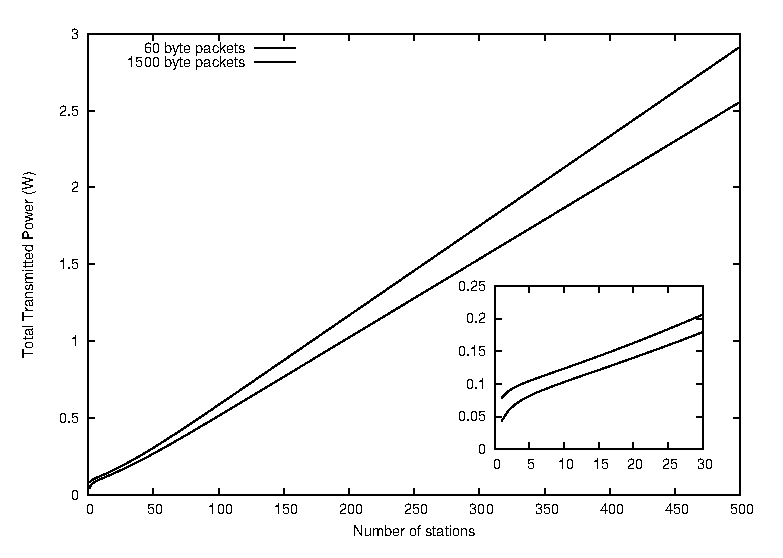
\includegraphics[width=30cm]{power3}
\end{center}


}
\end{pcolumn}
%%%%%%%%%%%%%%%%%%%%%%
\begin{pcolumn}{0.49}
\pbox{0.9\textwidth}{28cm}{linewidth=2mm,framearc=0.1,linecolor=lightblue,fillstyle=gradient,gradangle=0,gradbegin=white,gradend=white,gradmidpoint=1.0,framesep=1em}{

\medskip
%%% Introduction
\begin{center}\pbox{0.8\textwidth}{}{linewidth=2mm,framearc=0.1,linecolor=lightblue,fillstyle=gradient,gradangle=0,gradbegin=white,gradend=whiteblue,gradmidpoint=1.0,framesep=1em}{\begin{center}Conclusions, Future and Related Work\end{center}}\end{center}\vspace{1.25cm}

\smallskip

Conclusions:
\begin{itemize}
\item ICNIRP guideline: 80mW kg$^{-1}$ for the general public.
\item ICNIRP guideline: 400mW kg$^{-1}$ for occupational exposure.
\item This is whole body exposure limits for long time periods.
\item Even large unicast networks should not violate limits.
\item Broadcast network effectively disables 802.11's backoff.
\item Close for small person, but saturated all-broadcast network unrealstic.
\end{itemize}

\medskip

Future Work:
\begin{itemize}
\item Experimental validation.
\item Study of unsaturated networks.
\end{itemize}

\medskip

Related work:
\begin{itemize}
\item \emph{Radiofrequency Exposure from Wireless LANs Utilizing Wi-Fi Technology}, Kenneth R. Foster, Health Physics, March 2007, 93(3), 280--289.  

\item \emph{Exposure of the general public due to wireless {LAN} applications in public places}, G. Schmid et al, Radiation Protection Dosimetry, 2007, 124(1), 48--52.
\end{itemize}



}
\end{pcolumn}
\end{center}

\end{poster}

\end{document}

